\documentclass[twoside]{article}
\input{ISC18-english.sty}
\usepackage{setspace}
%%%%%%%%%%%%%%%%%%%%%%%%%%%%  Make sure to compile twice for proper cross-references. %%%%%%%%%%%%%%%%%%%%%%%
%%%%%%% For proper display of references, compile the document twice. %%%%%%%%%%%%%%%%%%%%% 
%%%%%%%%%%%%%%% If using TeX Live, compile using pdflatex command %%%%%%%%%%%%%%%%%%%%%%%
\begin{document}
\thispagestyle{empty}
%%%%%%%%%%%%%%%%% Article title header  %%%%%%%%%%%%%%%%%%%%
\fancyhead[LE]{Bayesian  Local Sensitivity to Non-ignorability}
%%%%%%%%%%%%%%%%% Article authors header   %%%%%%%%%%%%%%%%%%%%
\fancyhead[RO]{E. Momeni Roochi}
\begin{center}
{
\includegraphics [height=25mm, width=150.3mm] {Images/isc18E}} \\
\vspace*{-1.8cm}
%\begin{center}
%\color{blue} 
%{\hspace{0.1cm}\rule{\textwidth}{1mm}}\\
%\end{center}
\vspace*{4cm}
%%%%%%%%%%%%%%%%% Article title  %%%%%%%%%%%%%%%%%%%%
{\Large \bf Bayesian  Local Sensitivity to Non-ignorability with General Missingness of  Outcomes and Covariates}\\
%%%%%%%%%%%%%%%%% Article authors and affiliations %%%%%%%%%%%%%%%%%%%%
{\bf
Elahe Momeni Roochi  \footnote[1]{{\bf Corresponding Author:} {\tt e\_momeniruchi@sbu.ac.ir }} \\
$^1$Department of Statistics, Faculty of Mathematical Sciences, Shahid Beheshti University, Tehran, Iran}
\end{center}
\rule{\textwidth}{0.2mm}\\
%%%%%%%%%%%%%%%%% Article abstract  %%%%%%%%%%%%%%%%%%%%
\noindent{\bf Abstract:}\\
A major concern in statistical analysis is missing data. Analysis frequently operates
under the presumption that missingness is ignorable when it occurs in the
study. It is critical to evaluate the effect of missingness on the most important
Bayesian inferences because ignorability is an untestable assumption in the absence
of data augmentation. Previously, in a Bayesian framework, the influence of
missing outcomes’ non-ignorability was studied using local sensitivity indices. In
this paper, for the first time, the Bayesian  index of local
sensitivity to non-ignorability for data exposed to general missingness in 
outcome and covariates will be extended. My results indicate that the Bayesian estimates of parameters of interest via local sensitivity approximation are more accurate than complete-case analysis and ignorable model. I will evaluate
the features of my proposed indices through several simulated studies.
 
\noindent{\bf Keywords:} 
Local Sensitivity to Non-ignorability, General Missingness, Bayesian Approach, and Local Sensitivity Indices.\\
%\noindent{\bf Mathematics Subject Classification (2010):} $\rm 99X99$, $\rm 99X99$, $\rm 99X99$. \\
\hspace{1cm}\rule{\textwidth}{0.2mm}\\
%%%%%%%%%%%%%%
\section{Introduction}
The selection model pertaining to incomplete data articulates the joint distribution of the hypothetical complete data alongside the indicators of missingness as the marginal distribution of the complete data multiplied by the distribution of the missingness indicators conditioned on the complete data. The latter component is referred to as the missingness mechanism. \cite{Rubin:1976} clarified the conditions under which it is permissible to disregard the stochastic characteristics of the missingness mechanism without jeopardizing the integrity of model-based inferences: Missing at random (MAR) posits that the occurrence of missingness is independent of the values of the missing items, whereas parameter distinctness (PD) contends that the parameters that dictate the distribution of the hypothetical complete data and those that govern the missingness mechanism reside within a factorizable parameter space (for likelihood inference) or are a priori independent (for Bayesian inference). The conjunction of MAR and PD ensures the ignorability of the missingness mechanism in both likelihood-based and Bayesian inferential frameworks.
Analyses that disregard the intricacies of the missing data mechanism consequently presuppose, either implicitly or explicitly, an MAR  framework alongside a PD Parameterization   \citep{Little:1992, Little:Rubin:2002,Paik:Sacco:2000,Satten:Carroll:2000}. A significant concern is that the presumption of MAR is often not tenable across numerous practical applications; furthermore, it is not feasible to evaluate this assumption in a robust manner by solely scrutinizing the available data.

Typical selection models incorporate a nonignorability parameter that dictates the dependence of the probability of missingness on the values of the notional underlying data. It is customary to parameterize such models in a manner that renders the missingness mechanism MAR when the nonignorability parameter is assigned a value of 0. Estimating such a parameter is rarely feasible without the imposition of strong assumptions, and even under such circumstances, the resulting inferences may exhibit nonrobustness and pose computational challenges \citep{Diggle:Kenward:1994,Robins:et:als:2000,Scharfstein:et:al:2003}. Sensitivity analysis endeavors to mitigate this issue by deriving estimates of the other parameters across a spectrum of presumed values for the nonignorability parameter; should the estimates exhibit robustness to variations in its value, one concludes that the results are insensitive.
A local sensitivity analysis investigates the impact on inferences of small departures from MAR   assumption \citep{Troxel:et:al:2004,Zhang:Heitjan:2007,Eftekhari:2018,Momeni:Eftekhari:2024}. %To date, such analyses have primarily addressed scenarios wherein the absence of data is confined to outcome variables.
 Most of these analyses have primarily addressed scenarios wherein the missing  data is confined to outcome variables and  postulate a singular scalar non-ignorability parameter, thus facilitating a more straightforward interpretation. \cite{Gao:et:al:2016} considered the missingness  in both outcome and covariate simultaneously, but in the real world of data missingness is often in a general form, that is in some cases response variable is missed but the covariate is observed and vice versa. To date, in Bayesian approach there is no literature on local sensitivity analysis in the presence of  general missingness of outcome and covariates.  In this article, I extend the ISNI (index of sensitivity to local nonignorability) approach of \cite{Zhang:Heitjan:2007}, \cite{Gao:et:al:2016} and  \cite{Momeni:Eftekhari:2024}  in two directions: 1) I allow general missingness in outcomes and covariates which is not necessarily simultaneous. 2)  I use a Bayesian approach that incorporates prior information. 

In Section 2, I derive the Bayesian sensitivity indices. In Section 3, I conduct a simulation study to  evaluate the performance of these indices. Section 4 offers further discussion.
 
 
\section{Bayesian Local Sensitivity}
This section develops the Bayesian ISNI,  for general missingness in response and covariates. It presents the log-likelihood function, log-posterior function and proposes the Bayesian local  sensitivity indices.

\subsection{The log-likelihood and log-posterior function  }
The dataset comprises $N$ independent vectors $(Y_i,X_i,Z_i)$, wherein $Y_i$ represents an outcome that is subject to missingness, while $X_i$ is a covariate also afflicted by missingness, and $Z_i$ denotes a covariate vector that is devoid of any missingness. The variables $R_i$ and $S_i$ serve as indicators of missingness: $R_i = 1(0)$ if $Y_i$ is observed (missing); $S_i= 1(0)$ if $X_i$ is observed (missing). We can readily extend the definitions of $R_i$ and $S_i$ to vector forms in the context of multivariate $Y_i$ and $X_i$.
For simplicity
we factor the conditional distribution of $(R_i,S_i, Y_i, X_i)$
given $Z_i$ as
$
f_{\xi,\gamma,\pmb\theta_y,\pmb\theta_x}^{R_i,S_i,Y_i,X_i\mid Z_i}(r_i, s_i, y_i, x_i\mid z_i)=f_\xi^{R_i\mid S_i,Y_i,X_i,Z_i}(r_i\mid s_i,y_i,x_i, z_i)\times f_\gamma ^{S_i\mid Y_i,X_i,Z_i}(s_i\mid y_i,x_i, z_i)\times
 f_{\pmb\theta_y}^{Y_i\mid X_i,Z_i}(y_i\mid x_i, z_i)\times f_{\pmb\theta_x}^{X_i\mid Z_i}(x_i\mid z_i)
$
and henceafter write $f_{\pmb\theta_y}^{Y_i\mid X_i,Z_i}(y_i\mid x_i, z_i)$, $f_{\pmb\theta_x} ^{X_i\mid Z_i}$ as $f_{\pmb\theta_y}$, $f_{\pmb\theta_x}$, respectively. In addition, I denote the probabilities that $Y_i$ and $X_i$ are observed as, respectively,
\begin{small}
\begin{align}\label{Ymechanism}
f_\xi^{R_i\mid S_i,Y_i,X_i,Z_i}(1\mid s_i,y_i,x_i, z_i) = 
     \begin{cases}
       h(q_{\xi}(.)+\xi_{y}y_i) &\quad\text{if}\quad s=1\\
       h(q_{\xi}(.)+\xi_{x}x_i+\xi_{y}y_i) &\quad\text{if}\quad s=0 \\
     \end{cases}
\end{align}
\end{small}
\begin{small}
\begin{align}\label{Xmechanism}
f_\gamma ^{S_i\mid Y_i,X_i,Z_i}(1\mid y_i,x_i, z_i)=
 \begin{cases}
       h(q_{\gamma}(.)+\gamma_{y}y_i) &\quad\text{if}\quad r=1\\
       h(q_{\gamma}(.)+\gamma_{x}x_i+\gamma_{y}y_i) &\quad\text{if}\quad r=0 \\
     \end{cases}
\end{align}
\end{small}
where $h(.)$ is the inverse of an appropriate link function and $q_{\xi}(.)$ and $q_{\gamma}(.)$ are identifiable functions of observed values. In addition, $\pmb\nu=(\xi_{y},\xi_{x},\gamma_{x},\gamma_{y})^{T}$ is the vector of non-ignorability parameters. The assumption $\pmb\nu=\mathbf{0}$ leads to the MAR
missingness mechanism, which results in the ignorable model.
%and henceafter write $f_\xi^{R_i\mid S_i,Y_i,X_i,Z_i}$,
%$f_\gamma ^{S_i\mid Y_i,X_i,Z_i}$, $f_\pmb\theta^{Y_i\mid X_i,Z_i}(y_i\mid x_i, z_i)$, $f_\beta ^{X_i\mid Z_i}$ as $f_\xi$, $f_\gamma$, $f_\pmb\theta$, $f_\beta$, respectively. The log-likelihood is
The log-likelihood is then
\begin{small}\begin{align}
l&=\sum_{i:g_i=1,s_i=1}\bigg\{ln~(h(q_{\xi}(.)+\xi_{y}y_i))+ln~(h(q_{\gamma}(.)+\gamma_xx_i))+ln ~ f_{\pmb\theta_y}(y_i\mid x_i, z_i)+ln ~ f_{\pmb\theta_x}(x_i\mid z_i)\bigg\}\nonumber\\
&+\sum_{i:g_i=0,s_i=1}ln\bigg\{ \int \left( 1-h(q_{\xi}(.)+\xi_{y}y_{i}^{miss})\right)\times h(q_{\gamma}(.)+\gamma_{x}x_i+\gamma_{y}y_{i}^{miss})\nonumber\\
& \qquad\qquad\qquad\qquad \times f_{\pmb\theta_y}(y_{i}^{miss}\mid x_i, z_i)\times f_{\pmb\theta_x}(x_i\mid z_i)dy_{i}^{miss}\bigg\}\nonumber\\
&+\sum_{i:g_i=1,s_i=0}ln\bigg\{ \int  h(q_{\xi}(.)+\xi_{x}x_{i}^{miss}+\xi_{y}y_i)\times (1-h(q_{\gamma}(.)+\gamma_{y}y_i))\nonumber\\
& \qquad\qquad\qquad\qquad \times f_{\pmb\theta_y}(y_{i}\mid x_{i}^{miss}, z_i)\times f_{\pmb\theta_x}(x_{i}^{miss}\mid z_i)dx_{i}^{miss}\bigg\}\nonumber\\
&+\sum_{i:g_i=0,s_i=0}ln\bigg\{ \int \int (1-h(q_{\xi}(.)+\xi_{x}x_{i}^{miss}+\xi_{y}y_{i}^{miss}))\times (1- h(q_{\gamma}(.)+\gamma_{x}x_{i}^{miss}+\gamma_{y}y_{i}^{miss}))\nonumber\\
& \qquad\qquad\qquad\qquad \times f_{\pmb\theta_y}(y_{i}^{miss}\mid x_{i}^{miss}, z_i)\times f_{\pmb\theta_x}(x_{i}^{miss}\mid z_i)dx_{i}^{miss}dy_{i}^{miss}\bigg\}
\label{Likelihood}
\end{align}\end{small}
The parameters of main interest $\pmb\theta_y$ index the conditional
distribution of the outcome $Y$ given covariates $(X, Z)$. The
rest are nuisance parameters: $\pmb\theta_x$ govern the distribution
of $X$ given $Z$; $(q_{\gamma}, \gamma_{x},\gamma_{y})$ governs the missingness mechanism
of $S$ given $(Y, X, Z)$; and $(q_{\xi}, \xi_{x},\xi_{y})$ governs the
missingness mechanism of $R$ given $(S, Y, X, Z)$.
Let $\mathbf{q}=(q_\xi,q_\gamma)$. To conduct Bayesian inference, the joint prior density function
$
\pi (\pmb\theta_y , \pmb\theta_x,\mathbf{q})=\pi(\pmb\theta_y , \pmb\theta_x)\pi(\mathbf{q}),
$
is assigned to the parameters of the response, missing covariate and ignorable
missing mechanism models. Implementing the Bayes theorem, the log-posterior  function of $(\pmb\theta_y , \pmb\theta_x,\mathbf{q})$ is
\begin{align}
ln~\pi(\pmb\theta_y,\pmb\theta_x,\mathbf{q} | y,x,z,r,s;\pmb\nu)\propto ln~\pi(\pmb\theta_y,\pmb\theta_x)+ln~\pi(\mathbf{q})+l(\pmb\theta_y,\pmb\theta_x, \mathbf{q} |y,x,z,r,s;\pmb\nu),\label{posterior density function}
\end{align}
where $l(.)$ is the log-likelihood function of   $(\pmb\theta_y,\pmb\theta_x, \mathbf{q})$ in a selection model, given in equation \eqref{Likelihood}. The above posterior distribution does not possess a closed-form solution due to the integrals with respect to the non-ignorability parameters; therefore, numerical methods are required.
When $\nu =\mathbf{0}$, equation \eqref{posterior density function} simplifies to the ignorable   posterior density function. Conversely, when using a non-ignorable Bayesian model for data analysis, the
posterior density function becomes complex due to the computation of integrals
involving missing response and covariates. This
leads to time-consuming calculations. This method is particularly useful when the assumption
of ignorability is questioned and a non-ignorable Bayesian model is used for data
analysis. 
 %\vspace{-1\baselineskip}
\subsection{Bayesian index of sensitivity to non-ignorability}
\cite{Zhang:Heitjan:2007}, \cite{Eftekhari:2018} and  \cite{Momeni:Eftekhari:2024} advocated for the execution of a sensitivity analysis by evaluating the variation of the Bayes estimator  of $\pmb\theta_y$ as a function of the nonignorability parameter in the neighbourhood of the missing at random  model. I extend this framework to encompass scenarios in which both dependent variables and independent variables may be missing by employing a first-order Taylor expansion of the Bayes estimator of $\pmb\theta_{y}$ under
squared error loss (S.E.L) given a fixed value of $\pmb\nu$ (i.e. $\hat{\pmb\theta}_{yB}(\pmb\nu)$) at $\pmb\nu =\mathbf{0}$:
\begin{align}\label{lin appr}
\hat{\pmb\theta}_{yB}(\pmb\nu)\simeq\hat{\pmb\theta}_{yB}(\mathbf{0})+\pmb\nu^T\frac{\partial \hat{\pmb\theta}_{yB}(\pmb\nu)}{\partial \pmb\nu}|_{\pmb\nu=\mathbf{0}},
\end{align}
where $\hat{\pmb\theta}_{yB}(\mathbf{0})$ is the ignorable Bayes estimator of $\pmb\theta_{y}$. Local sensitivity analysis considers whether small values
of the nonignorability parameter $\pmb\nu$ can yield nonnegligible
changes in the Bayes estimates. Following \cite{Zhang:Heitjan:2007}, I
define the index of local sensitivity to nonignorability as
$\pmb\Lambda^{1}(\pmb\theta _y)= \frac{\partial \hat{\pmb\theta}_{yB}(\pmb\nu)}{\partial \pmb\nu }\big|_{\pmb\nu=\mathbf{0}}$.
Then a general formula for
$\pmb\Lambda^{1}(\pmb\theta _y)$ is
\begin{footnotesize}\begin{align}\label{ISNI}
\pmb\Lambda^{1}(\pmb\theta_y)  = \begin{pmatrix}
    Cov_I(\pmb\theta_y,\frac{\partial l(\pmb\theta_y,\pmb\theta_x, \mathbf{q} |y,x,z,r,s;\pmb\nu)}{\partial \xi_y}\big|_{\pmb\nu=\mathbf{0}})           \\
   Cov_I(\pmb\theta_y,\frac{\partial l(\pmb\theta_y,\pmb\theta_x, \mathbf{q} |y,x,z,r,s;\pmb\nu)}{\partial \xi_x}\big|_{\pmb\nu=\mathbf{0}})\\
             Cov_I(\pmb\theta_y,\frac{\partial l(\pmb\theta_y,\pmb\theta_x, \mathbf{q} |y,x,z,r,s;\pmb\nu)}{\partial \gamma_x}\big|_{\pmb\nu=\mathbf{0}})\\ 
             Cov_I(\pmb\theta_y,\frac{\partial l(\pmb\theta_y,\pmb\theta_x, \mathbf{q} |y,x,z,r,s;\pmb\nu)}{\partial \gamma_y}\big|_{\pmb\nu=\mathbf{0}})
\end{pmatrix},
\end{align}\end{footnotesize}
Each element of the $\pmb\Lambda^{1}(\pmb\theta_y)$ vector in \eqref{ISNI} is the posterior covariance between the parameters \(\pmb\theta_y\) and the derivative of the non-ignorable log-likelihood with respect to a non-ignorability parameter, evaluated at \(\pmb\nu=0\). This covariance is typically intractable but can be approximated numerically.
\section{Simulation Study}
%%%%%%%%%%%%%%%%%%%%%%%%%%%%%%% Unnumbered formula %%%%%%%%%%%%%%%%%%%%%%%
 I apply ISNI to some simulated
datasets from the Bayesian simple linear regression model with the possibility of general  missing outcome and covariate.

Without any loss of generality, I will consider a linear regression
model that includes a single normally distributed covariate with the possibility of
general missingness with the response variable. Therefore, $Y_i$ and $X_i$ follow a bivariate normal distribution, represented as $(Y_i,X_i)^T\sim N_2(\pmb\mu,\pmb\Sigma)$, with the mean vector $\pmb\mu=(\beta_0+\beta_1\mu_x,\mu_x)^T$ and the covariance matrix $\pmb\Sigma=
\begin{pmatrix}
\sigma^2_{y}& \beta_1\sigma^2_x \\
\beta_1\sigma^2_x & \sigma^2_x
\end{pmatrix}$,     
where $Y_i $ and $X_i$ are the outcome  and  covariate for the $i$th subject, respectively. $\beta_0$ and $\beta_1$ represent regression coefficients, whereas the marginal variance of $Y$ is calculated as $\sigma^2_{y}=\beta_{1}^2 \sigma^2_x+\sigma^2_{y\mid x}$, where $\sigma^2_{y\mid x}$ and $\sigma^2_{x}$ denote the variances of the conditional distribution of $Y$ given $X$, and the marginal distribution of $X$, respectively. Some random samples, each with a size of $N=500$ are generated. The random samples are  simulated based on the aforementioned simple linear regression model with the set of true parameter values  $\beta_0=1$, $\beta_1=2$, $\sigma^2_{y\mid x}=\sigma^2_x=1$ and $\mu_x=0$. Additionally,  missing values in both the outcome and covariate are generated using equations \eqref{Ymechanism} and \eqref{Xmechanism} with a logit link function. For simplicity, I consider  $q_\xi(.)=\alpha_{01y}$ and $q_\xi(.)=\alpha_{02y}$ for the first and second equations of \eqref{Ymechanism}, respectively. Furthermore, $q_{\gamma}(.)=\alpha_{0x}$ in \eqref{Xmechanism}. To conduct Bayesian inference, the Jeffreys’ prior for $(\pmb\mu,\pmb\Sigma)$ and  non-informative
prior $N(0,10^3)$ is considered for $\alpha_{01y}$, $\alpha_{02y}$ and $\alpha_{0x}$. The posterior samples are obtained via Independent Metropolis-Hastings algorithm with multivariate multivariate normal proposal distribution. The location parameter of this proposal distribution is assumed to be the ML estimate of parameters
$\beta_0$, $\beta_1$, $\sigma^2_{y\mid x}$, $\sigma^2_x$, $\alpha_{0x}$, $\alpha_{01y}$ and $\alpha_{02y}$ , and the scale parameter is  the inverse of the negative Hessian matrix. I generated 50000 MCMC samples along with 20000 burn-ins.
A range of different missing rates is obtained by specifying distinct values for $\alpha_{01y}$, $\alpha_{02y}$ and $\alpha_{0x}$ within the missingness mechanisms \eqref{Ymechanism} and \eqref{Xmechanism}. These values are set as follows: 1)$\alpha_{01y}=1$, $\alpha_{02y}=-0.9$, $\alpha_{0x}=-0.5$, 2) identical to setting 1, with the exception of $\alpha_{01y}=0.5$, 3) identical to setting 1, with the exception of $\alpha_{01y}=1.5$, 4) identical to setting 1, with the exception of $\alpha_{0x}=0.5$, 5) identical to setting 1, with the exception of $\alpha_{0x}=1$, 6) identical to setting 1, with the exception of $\alpha_{0x}=1.5$, 7) identical to setting 1, with the exception of $\alpha_{0x}=2$, 8) identical to setting 1, with the exception of $\alpha_{0x}=2.5$. In addition, the true values of the vector of non-ignorability parameters, $\nu$, are set as $(-0.3,1,-0.8,2)$.  To obtain reliable results, each missingness occurrence scenario   was repeated 100 times. In each repetition, the values of $\pmb\Lambda^{1}(\pmb\theta _y)$ in \eqref{ISNI} are calculated for parameters of $\beta_0$ and $\beta_1$. Subsequently,  the approximate Bayesian estimates for these parameters are calculated using the first$-$order  Taylor expansion \eqref{lin appr}. For comparison, Bayesian estimates via complete$-$case analysis and an ignorable model are also obtained.
Table \ref{table1} 
presents the average missing rates in the covariate (Xrate) and response (Yrate), along with the absolute biases of the Bayesian estimates under complete$-$case analysis, the ignorable model (ign) and  the first$-$order Taylor expansion approximation (appr) of $\pmb\theta_y=(\beta_0 , \beta_1)$. The posterior standard errors of Bayesian estimates (sd) are also shown. According to these tables,   the biases of the Bayesian estimates obtained by  the first$-$order Taylor expansion approximation are, on average,  clearly smaller than those of the other methods, indicating the superiority of ISNI.
\setlength{\textfloatsep}{4pt}
\setlength{\tabcolsep}{4pt}
\begin{table}[h] %
  \centering
  \begin{scriptsize}
  \caption{\small Average results of Bayesian  parameter estimation and approximate estimates  via first-order Taylor expansion in Bayesian local sensitivity analysis of $\beta_0$ and $\beta_1$  for eight simulated datasets with N = 500 individuals, in different missing rates}\label{table1}
    \begin{tabular}{|c|cc|ccccc|ccccc|}
     \hline
          &    Missing   &    Rate   &       &       & $\beta_0$ &       &       &       &       & $\beta_1$ &       &  \\ \hline
         Scenario & Xrate & Yrate & Bias.cc & sd.cc & Bias.ign & sd.ign & Bias.appr &  Bias.cc & sd.cc & Bias.ign & sd.ign & Bias.appr \\\hline \hline
    1     & 0.376 & 0.382 & 0.451 & 0.089 & 0.427 & 0.101 & 0.354 & 0.549 & 0.096 & 0.249 & 0.092 & 0.042 \\
    2     & 0.404 & 0.418 & 0.575 & 0.094 & 0.479 & 0.122 & 0.040 & 0.425 & 0.091 & 0.250 & 0.092 & 0.062 \\
    3     & 0.432 & 0.338 & 0.404 & 0.080 & 0.285 & 0.087 & 0.197 & 0.596 & 0.089 & 0.145 & 0.082 & 0.006 \\
    4     & 0.282 & 0.328 & 0.432 & 0.068 & 0.201 & 0.077 & 0.305 & 0.568 & 0.078 & 0.149 & 0.075 & 0.009 \\
    5     & 0.248 & 0.312 & 0.279 & 0.070 & 0.250 & 0.072 & 0.199 & 0.721 & 0.073 & 0.117 & 0.067 & 0.065 \\
    6     & 0.252 & 0.168 & 0.276 & 0.064 & 0.317 & 0.068 & 0.046 & 0.724 & 0.069 & 0.196 & 0.065 & 0.060 \\
    7     & 0.230 & 0.192 & 0.193 & 0.055 & 0.245 & 0.057 & 0.030 & 0.807 & 0.061 & 0.108 & 0.057 & 0.101 \\
    8     & 0.206 & 0.162 & 0.282 & 0.057 & 0.203 & 0.062 & 0.132 & 0.718 & 0.066 & 0.100 & 0.063 & 0.071 \\\hline
    \end{tabular}%
  \end{scriptsize}
\end{table}%
To explore these superiority, figure \ref{fig1} shows the boxplot of the biases obtained in eight scenarios for each method and parameter. This figure indicates that the biases of first-order Taylor expansion approximation are smaller than other methods.
\begin{figure}[ht]
\begin{center}
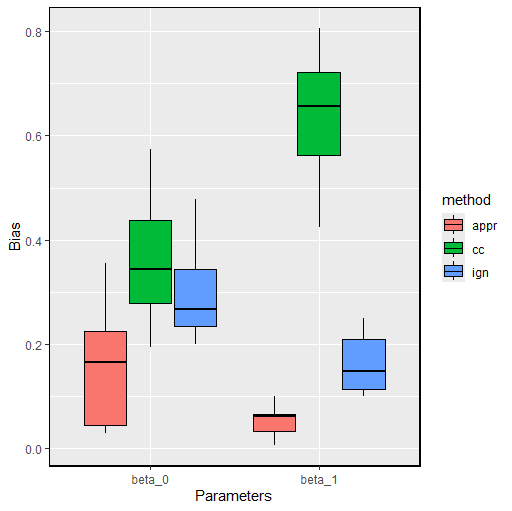
\includegraphics[width=7cm,height=6cm]{Images/boxplot.png}
\vspace{-0.2cm}
\caption{\footnotesize{Comparison of absolute values of biases of Bayesian estimates in complete$-$case (cc) and ignorable  (ign) analysis with the   first-order Taylor expansion approximation (appr) of $\beta_0$ and $\beta_1$ in eight simulated datasets.}}\label{fig1}
\end{center}
\end{figure}


\section{Discussion  and Conclusions}
This paper has introduced novel Bayesian local sensitivity indices to address
the critical, yet understudied, problem of non-ignorable general missingness,
where the response variable and  covariates are missing that is not necessarily simultaneous.
 The proposed  indices, $\pmb\Lambda^{1}(\pmb\theta _y)$  efficiently quantify the sensitivity of posterior estimates locally around the more tractable ignorable (MAR) model. This provides a powerful diagnostic
tool for a complex missing data problem without requiring the fitting of a full
non-ignorable model.

My extensive simulation studies, designed specifically around scenarios of general
missingness in simple  linear regression, demonstrate that
the Bayesian estimates via ISNI are more accurate than other methods like complete$-$case analysis and ignorable model.

An important limitation of the current work, as with most local sensitivity
approaches, is its reliance on the correct parametric specification of the selection
model. A promising extension to mitigate this
limitation would be to develop my index within a more flexible, semiparametric
Bayesian selection model, building on recent advances in this area \cite{Sugasawa:et:al:2022}. This would enhance the robustness of
the sensitivity analysis to parametric assumptions.
\begin{thebibliography}{9}
\begin{spacing}{1}
\bibitem[Diggle and Kenward (1994)]{Diggle:Kenward:1994}
Diggle P. and Kenward  M.G. (1994), Informative drop-out in longitudinal
data analysis, {\it J. R. Stat. Soc., C: Appl. Stat.}
43, 49–73.

\bibitem[Eftekhari Mahabadi (2018)]{Eftekhari:2018}
Eftekhari Mahabadi S. (2018), Second‐order local sensitivity to non‐ignorability
in Bayesian inferences, {\it Stat. Med.} 37, 3616–3636.

\bibitem[Gao et al. (2016)]{Gao:et:al:2016}
Gao W., Hedeker D., Mermelstein R. and Xie H. (2016), A scalable approach
to measuring the impact of nonignorable nonresponse with an ema application,
{\it Stat. Med.} 35, 5579–5602.

\bibitem[Little (1992)]{Little:1992}
Little R.J.A. (1992), Regression with missing X's: a review, {\it J. Am. Stat. Assoc.} 87,  1227–1237.

\bibitem [Little and Rubin (2002)]{Little:Rubin:2002}
Little R. and Rubin D. (2002), {\it Statistical analysis with missing data, 2 edn,}
 New York, John Wiley.
 
\bibitem[Momeni Roochi  and Eftekhari Mahabadi  (2024)]{Momeni:Eftekhari:2024}
Momeni Roochi E. and Eftekhari Mahabadi S. (2024), Bayesian second-order
sensitivity of longitudinal inferences to non-ignorability: an application to antidepressant
clinical trial data, {\it Int. J. Biostat.} 20, 599-629.
 
 \bibitem [Paik and Sacco (2000)]{Paik:Sacco:2000}
Paik M.C. and Sacco R.L. (2000), Matched case-control data analyses
with missing covariates, {\it J. R. Stat. Soc., C: Appl. Stat.} 49, 145–156.

\bibitem[Robins et al. (2000)]{Robins:et:als:2000}
Robins J.M., Rotnitzky A. and Scharfstein D.O. (2000), Sensitivity
analysis for selection bias and unmeasured confounding in missing
data and causal inference models. In: {\it Halloren, M.E. and Berry,
D. (Eds.) Statistical models in epidemiology, the environment, and
clinical trials,} Springer, pp. 1–94.

\bibitem[Rubin (1976)]{Rubin:1976}
Rubin D.B. (1976), Inference and missing data, {\it Biometrika} 63,  581–
592.

\bibitem[Satten  and Carroll  (2000)]{Satten:Carroll:2000}
Satten G.A. and Carroll R.J. (2000), Conditional and unconditional categorical
regression models with missing covariates, {\it Biometrics} 56,
384–388.


\bibitem[Scharfstein et al. (2003)]{Scharfstein:et:al:2003}
Scharfstein D.O., Daniels M.J. and Robins J.M. (2003), Incorporating
prior beliefs about selection bias into the analysis of randomized
trials with missing outcomes, {\it Biostatistics} 4, 495–512.
 

\bibitem[Sugasawa et al. (2022)]{Sugasawa:et:al:2022}
Sugasawa S., Morikawa K. and Takahata K. (2022), Bayesian semiparametric
modeling of response mechanism for nonignorable missing data, {\it Test}
31, 101–117.

\bibitem[Troxel et al. (2004)]{Troxel:et:al:2004}
Troxel A.B., Ma G. and Heitjan D.F. (2004), An index of local sensitivity
to nonignorability, {\it Stat. Sin.} 14, 1221–1237.

\bibitem[Zhang and Heitjan (2007)]{Zhang:Heitjan:2007}
Zhang J. and Heitjan D. (2007), Impact of nonignorable coarsening on Bayesian
inference, {\it Biostatistics} 8, 722–743.
\end{spacing}
\end{thebibliography}
 \end{document}

